\documentclass[12pt]{article}

\usepackage[a4paper,left=25mm,right=25mm,top=35mm,bottom=25mm]{geometry}
\usepackage{ngerman}
\usepackage{parskip}
\usepackage{times}
\usepackage{graphicx}
\usepackage{listings}
\usepackage{fancyhdr}
\usepackage{float}

\setlength{\headheight}{15.2pt}
\pagestyle{fancy}

\lhead{Bildverarbeitung und Mustererkennung\\Praktikum Blatt 3}
\rhead{Patrick Hüntelmann\\06.05.2022}

\lstset{
  basicstyle=\ttfamily,
  breakatwhitespace=false,         % sets if automatic breaks should only happen at whitespace
  breaklines=true,                 % sets automatic line breaking
  captionpos=b,                    % sets the caption-position to bottom
  deletekeywords={...},            % if you want to delete keywords from the given language
  escapeinside={\%*}{*)},          % if you want to add LaTeX within your code
  extendedchars=true,              % lets you use non-ASCII characters; for 8-bits encodings only, does not work with UTF-8
  frame=single,	                   % adds a frame around the code
  keepspaces=true,                 % keeps spaces in text, useful for keeping indentation of code (possibly needs columns=flexible)
  language=python,                 % the language of the code
  showstringspaces=false,          % underline spaces within strings only
  showtabs=false,                  % show tabs within strings adding particular underscores
  tabsize=2,	                   % sets default tabsize to 2 spaces
}

\begin{document}

\pagenumbering{arabic}

\section*{Aufgabe 3}
\subsection*{Teil 1. Lineare Filter}
Die Anwendung des Mittelwertfilter ist in der Funktion \textbf{filter\_average} (main.py Zeile 86) implementiert, welche als Parameter das Bild (\textbf{img}) und den Skalar $n$ übergeben bekommt.
Die Funktion generiert mit der Funktion \textbf{generate\_average\_mask} eine Maske der Größe $(2n+1)^2$, bei der jedes Element den Wert $\frac{1}{(2n+1)^2}$ hat, und ruft anschließend die Funktion \textbf{apply\_linear\_filter} auf, welche dann das Ergebnisbild zurückgibt.

Die Anwendung des Binominalfilters ist in der Funktion \textbf{filter\_binominal} (main.py Zeile 91) implementiert, diese Funktion ist sehr Ähnlich aufgebaut generiert aber mit der Funktion \textbf{generate\_binominal\_mask} die Maske für die Binominalfilterung und wendet diese dann auf dem Bild an.

\subsubsection*{Ergebnisbilder}
\begin{figure}[H]
  \centering
  \begin{minipage}{0.49\textwidth}
    \centering
    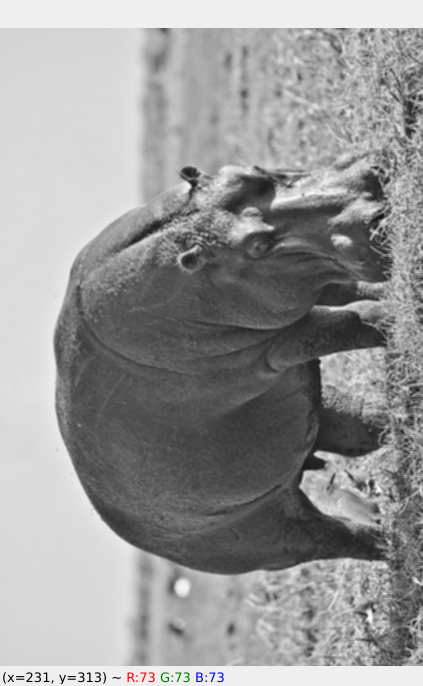
\includegraphics[width=\textwidth, height=0.4\textheight, keepaspectratio]{average_1.png}
    Mittelwertfilter ($n = 1$)
  \end{minipage}
  \hfill
  \begin{minipage}{0.49\textwidth}
    \centering
    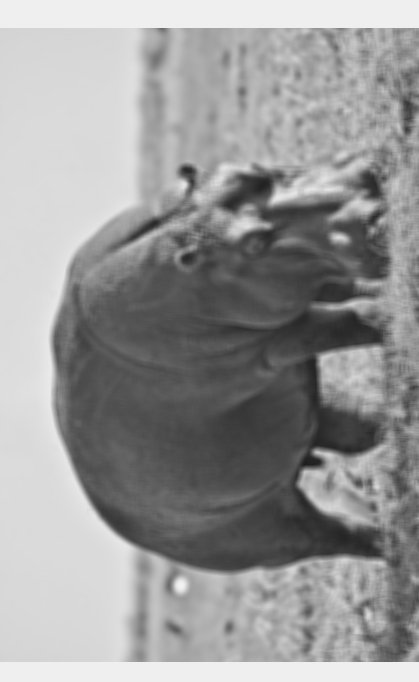
\includegraphics[width=\textwidth, height=0.4\textheight, keepaspectratio]{average_3.png}
    Mittelwertfilter ($n = 3$)
  \end{minipage}
\end{figure}
\begin{figure}[H]
  \centering
  \begin{minipage}{0.49\textwidth}
    \centering
    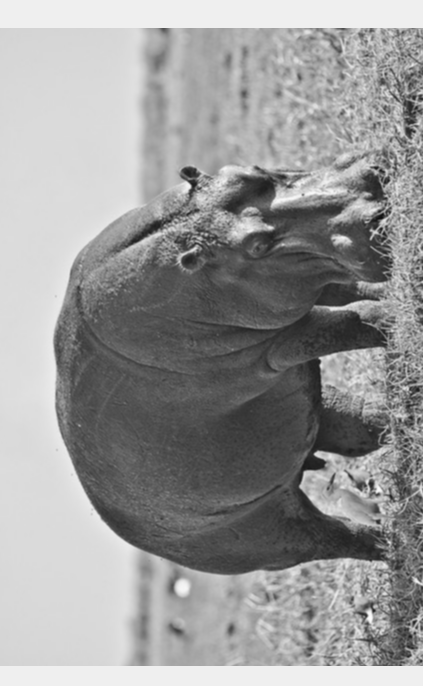
\includegraphics[width=\textwidth, height=0.4\textheight, keepaspectratio]{binominal_1.png}
    Binominalfilter ($n = 1$)
  \end{minipage}
  \hfill
  \begin{minipage}{0.49\textwidth}
    \centering
    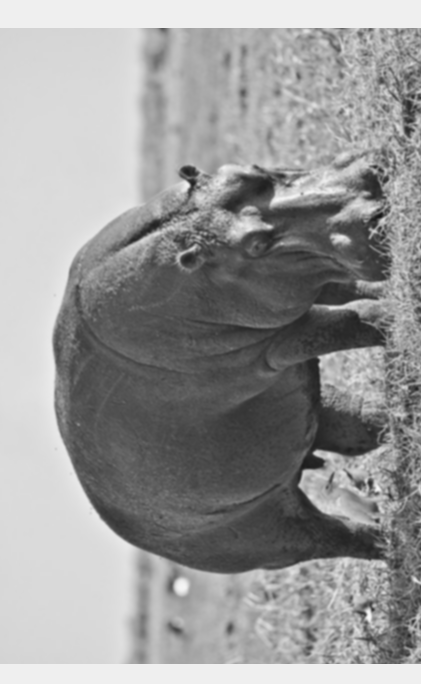
\includegraphics[width=\textwidth, height=0.4\textheight, keepaspectratio]{binominal_2.png}
    Binominalfilter ($n = 2$)
  \end{minipage}
\end{figure}
\newpage

\subsection*{Teil 2: Gewichteter Medianfilter}
Die Anwendung des gewichteten Medianfilters ist in der Funktion \textbf{apply\_median\_filter} (main.py Zeile 74) implementiert, welche als Parameter das Bild (\textbf{img}) und die Gewichtung (\textbf{weights}) übergeben bekommt.
Diese Funktion iteriert durch die Blöcke des Bildes und ruft die Funktion \textbf{calculate\_median\_filter}, welche jeden Bildpunkt mit der entsprechenden Gewichtung multipliziert und den Medianwert diesem Ergebnis zurückgibt.

\subsubsection*{Ergebnisbild}
\begin{figure}[H]
  \centering
  \begin{minipage}{0.49\textwidth}
    \centering
    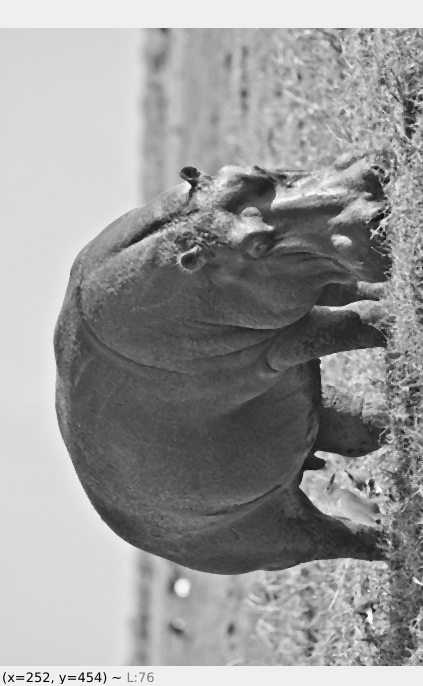
\includegraphics[width=\textwidth, height=0.6\textheight, keepaspectratio]{median_1.png}
    Medianfilter ($n = 1$)
  \end{minipage}
\end{figure}

\end{document}
